\documentclass[12pt]{article}
\usepackage{mathtools,amssymb, amsthm, tikz}
\usetikzlibrary{patterns}
\usepackage[margin=1in]{geometry}
\usepackage{url}
\usepackage{natbib}
\usepackage[colorlinks=true, linkcolor=black, urlcolor=blue, citecolor=blue]{hyperref}
\usepackage[T1]{fontenc}
\usepackage[utf8]{inputenc}
\usepackage{lmodern}

\title{Edge Function}
\author{Pintér Bálint}
\renewcommand{\contentsname}{Tartalomjegyzék}
\renewcommand{\bibsection}{\section*{Források}}

\begin{document}
\maketitle
\newpage
\tableofcontents
\newpage

\section{Bevezetés}
Az edge function egy lineáris függvény, amellyel egy egyenessel kettéosztott
síkon lévő pontokat lehet három régióba osztani:
\begin{itemize}
    \item Az egyenestől 'jobbra' lévő pontok (ahol a függvény értéke pozitív).
    \item Az egyenestől 'balra' lévő pontok (ahol a függvény értéke negatív).
    \item Az egyenesre illeszkedő pontok (ahol a függvény értéke nulla).
\end{itemize}
\begin{center}
    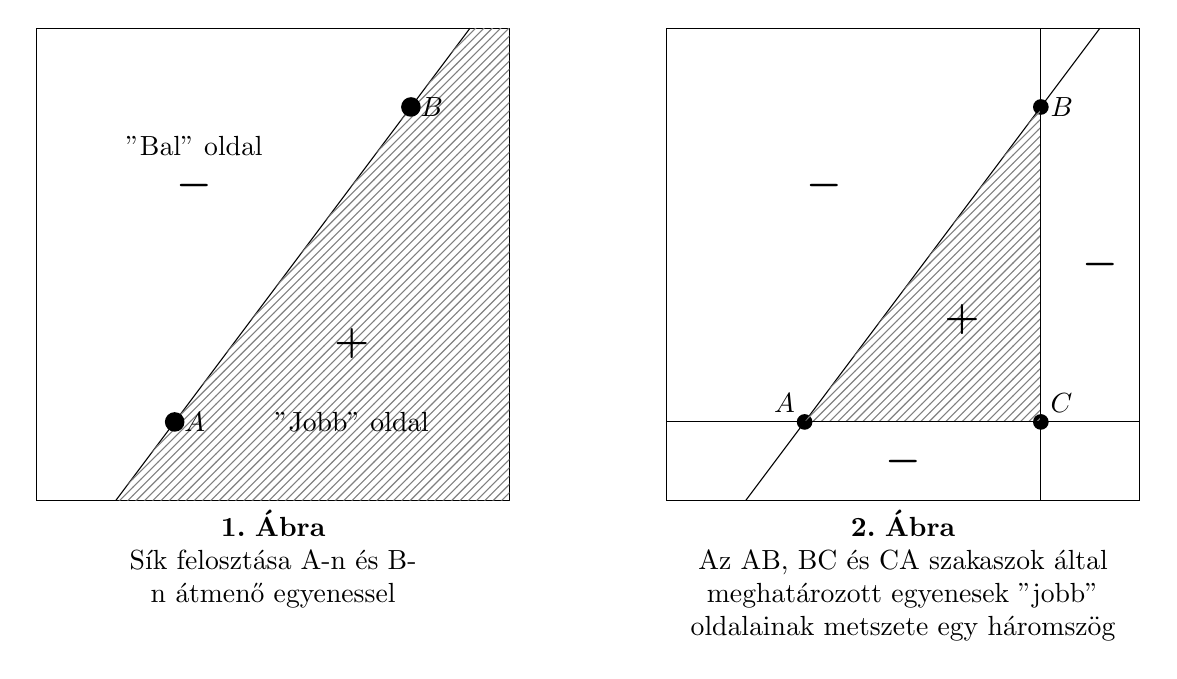
\begin{tikzpicture}
        \coordinate (BL1) at (0,0);
        \coordinate (BR1) at (6,0);
        \coordinate (TR1) at (6,6);
        \draw (BL1) rectangle (TR1);
        \coordinate (B1) at (1,0);
        \coordinate (T1) at (5.5,6);
        \draw (B1) -- (T1);
        \fill[pattern=north east lines, pattern color=gray]
        (T1) -- (TR1) -- (BR1) -- (B1) -- cycle;

        \coordinate (A1) at (1.75,1);
        \node[circle, fill, inner sep=2.5pt] at (A1) {};

        \coordinate (B1) at (4.75,5);
        \node[circle, fill, inner sep=2.5pt] at (B1) {};

        \node[right] at (A1) {$A$};
        \node[right] at (B1) {$B$};
        \node[font=\Large] at (2,4) {$\boldsymbol{-}$};
        \node[] at (2,4.5) {"Bal" oldal};
        \node[font=\Large] at (4,2) {$\boldsymbol{+}$};
        \node[] at (4, 1) {"Jobb" oldal};
        \node[below, text width=6cm, align=center] at (3,0) {\textbf{1.~Ábra}\\Sík felosztása A-n és B-n átmenő egyenessel};

        \coordinate (BL2) at (8,0);
        \coordinate (BR2) at (14,0);
        \coordinate (TR2) at (14,6);
        \draw (BL2) rectangle (TR2);
        \coordinate (B2) at (9,0);
        \coordinate (T2) at (13.5,6);
        \draw (B2) -- (T2);

        \coordinate (A2) at (9.75,1);
        \node[circle, fill, inner sep=2pt] at (A2) {};

        \coordinate (B2) at (12.75,5);
        \node[circle, fill, inner sep=2pt] at (B2) {};

        \coordinate (C2) at (12.75,1);
        \node[circle, fill, inner sep=2pt] at (C2) {};
        \draw (A2) -- (C2) -- (B2);
        \fill[pattern=north east lines, pattern color=gray]
        (A2) -- (B2) -- (C2) -- cycle;

        \draw (12.75,6) -- (12.75,0);

        \draw (8,1) -- (14,1);

        \node[font=\Large] at (10,4) {$\boldsymbol{-}$};

        \node[font=\Large] at (13.5,3) {$\boldsymbol{-}$};

        \node[font=\Large] at (11,0.5) {$\boldsymbol{-}$};

        \node[font=\Large] at (11.75,2.3) {$\boldsymbol{+}$};

        \node[above left] at (A2) {$A$};
        \node[right] at (B2) {$B$};
        \node[above right] at (C2) {$C$};
        \node[below, text width=6cm, align=center] at (11,0) {\textbf{2.~Ábra}\\Az AB, BC és CA szakaszok által meghatározott egyenesek "jobb" oldalainak metszete egy háromszög};

    \end{tikzpicture}
\end{center}
A 2. ábra szemlélteti, hogy a háromszög 'belseje' a három oldalhoz tartozó megfelelő irányú edge function előjelei alapján meghatározható.
\newpage
\section{Edge function levezetése}
\begin{itemize}
    \item Legyen a szakasz kezdőpontja $P_{0} = (X,Y)$
    \item Legyen a szakasz végpontja $P_{1} = (X + dX,Y + dY)$
          \begin{itemize}
              \item Ekkor a $\vec{P_{0}P_{1}}=\vec{v}=((X + dX) - X, (Y + dY) - Y)=(dX, dY)$
          \end{itemize}
    \item Legyen a vizsgált pont $P = (x,y)$
          \begin{itemize}
              \item Ekkor a $\vec{P_{0}P}=\vec{u}=(x - X, y - Y)$
          \end{itemize}
\end{itemize}
Az edge function lényegében egy 'keresztszorzat'. Kettő két dimenziós vektor
'keresztszorzata' a rájuk merőleges vektor $Z$ koordinátáját adja meg.
\begin{align*}
    \vec{u}\times\vec{x}=\det
    \begin{bmatrix}
        u_{x} & u_{y} \\
        v_{x} & v_{y}
    \end{bmatrix}
    = u_{x}v_{y}-v_{x}u_{y}
\end{align*}
Helyettesítsuk be az értékeinket:
\begin{align*}
    u_{x} &= x - X \\
    u_{y} &= y - Y \\
    v_{x} &= dX \\
    v_{y} &= dY \\
\end{align*}
A végeredmény:
\begin{align*}
    \boxed{E(x,y)=(x - X)dY-(y - Y)dX}
\end{align*}
\newpage
\section{Edge function működési elve}
\newpage
\nocite{*}
\bibliographystyle{plainnat}
\bibliography{forrasok}

\end{document}